\chapter{Final coefficients \label{sec:app:final_coefficients}}
\begin{table}[H]
    \centering
    \begin{tabular}{c|c|c|c}
         \thead{Coefficient} & \thead{Phase II} & \thead{Phase III} & \thead{Phases II + III} \\ \hline
         \makecell{$a^B$} & \makecell{1.02394} & \makecell{1.00341} & \makecell{1.03179} \\
         \makecell{$b^B$} & \makecell{1.08484} & \makecell{1.06898} & \makecell{1.07573} \\
         \makecell{$c^B$} & \makecell{1.18253} & \makecell{1.12627} & \makecell{1.16176} \\
         \makecell{$x_0^B$} & \makecell{-0.0344209} & \makecell{-0.0131757} & \makecell{-0.0269844} \\
         \makecell{$y_0^B$} & \makecell{0.22116} & \makecell{0.212521} & \makecell{0.219484} \\
         \makecell{$z_0^B$} & \makecell{-0.195463} & \makecell{-0.192554} & \makecell{-0.195859} \\
         \hline
         \makecell{$a^g$} & \makecell{0.969417} & \makecell{0.978286} & \makecell{0.97323} \\
         \makecell{$b^g$} & \makecell{0.959791} & \makecell{0.948732} & \makecell{0.957992} \\
         \makecell{$c^g$} & \makecell{0.964618} & \makecell{0.926156} & \makecell{0.953446} \\
         \makecell{$x_0^g$} & \makecell{-0.00218404} & \makecell{0.00733717} & \makecell{0.00149607} \\
         \makecell{$y_0^g$} & \makecell{-0.0149083} & \makecell{-0.0113024} & \makecell{-0.014287} \\
         \makecell{$z_0^g$} & \makecell{-0.0218019} & \makecell{-0.0260466} & \makecell{-0.0251443} \\
    \end{tabular}
    \caption{Coefficients determined from measurement on 11 April 2025.}
    \label{tab:app:coeff}
\end{table}

\begin{table}[H]
    \centering
    \begin{tabular}{c|c|c|c|c|c|c}
             &   xa0  &   ya0  &   za0  &   aa   &   ba   & ca \\
         xa0 &  1     &        &        &        &        &    \\
         ya0 & -0.005 &  1     &        &        &        &    \\
         za0 & -0.016 & -0.007 &  1     &        &        &    \\
         aa  &  0.522 & -0.000 & -0.005 &  1     &        &    \\
         ba  &  0.010 &  0.251 & -0.011 &  0.003 &  1     &    \\
         ca  & -0.008 & -0.015 &  0.273 & -0.007 & -0.013 &  1 \\
    \end{tabular}
    \caption{Correlation matrix of Phase II Acc}
\end{table}

\begin{table}[H]
    \centering
    \begin{tabular}{c|c|c|c|c|c|c}
             &   xm0  & ym0    &   zm0  &   am   &   bm   & cm \\
         xm0 &  1     &        &        &        &        &    \\
         ym0 &  0.096 &  1     &        &        &        &    \\
         zm0 & -0.114 & -0.013 &  1     &        &        &    \\
         am  &  0.457 &  0.055 & -0.105 &  1     &        &    \\
         bm  & -0.180 &  0.212 & -0.045 & -0.212 &  1     &    \\
         cm  & -0.229 & -0.065 &  0.282 & -0.252 & -0.093 & 1  \\
    \end{tabular}
    \caption{Correlation matrix of Phase II Mag}
\end{table}

\begin{table}[H]
    \centering
    \begin{tabular}{c|c|c|c|c|c|c}
             &   xa0  &   ya0  &   za0  &   aa   &   ba   & ca \\
         xa0 &  1     &        &        &        &        &    \\
         ya0 &  0.030 &  1     &        &        &        &    \\
         za0 & -0.093 & -0.017 &  1     &        &        &    \\
         aa  & -0.246 & -0.004 & -0.047 &  1     &        &    \\
         ba  & -0.021 & -0.034 &  0.055 & -0.229 &  1     &    \\
         ca  & -0.017 &  0.053 & -0.280 & -0.098 & -0.195 &  1 \\
    \end{tabular}
    \caption{Correlation matrix of Phase III Acc}
    \label{tab:my_label}
\end{table}

\begin{table}[H]
    \centering
    \begin{tabular}{c|c|c|c|c|c|c}
             &   xm0  & ym0    &   zm0  &   am   &   bm   & cm \\
         xm0 &  1     &        &        &        &        &    \\
         ym0 &  0.053 &  1     &        &        &        &    \\
         zm0 & -0.006 & -0.009 &  1     &        &        &    \\
         am  & -0.266 & -0.015 & -0.033 &  1     &        &    \\
         bm  &  0.013 &  0.073 &  0.014 & -0.234 &  1     &    \\
         cm  &  0.017 &  0.046 & -0.222 & -0.185 & -0.203 & 1  \\
    \end{tabular}
    \caption{Correlation matrix of Phase III Mag}
\end{table}

\begin{table}[H]
    \centering
    \begin{tabular}{c|c|c|c|c|c|c}
             &   xa0  &   ya0  &   za0  &   aa   &   ba   & ca \\
         xa0 &  1     &        &        &        &        &    \\
         ya0 & -0.001 &  1     &        &        &        &    \\
         za0 & -0.067 & -0.004 &  1     &        &        &    \\
         aa  &  0.283 & -0.008 & -0.049 &  1     &        &    \\
         ba  & -0.029 &  0.206 & -0.012 & -0.058 &  1     &    \\
         ca  & -0.053 & -0.008 &  0.127 & -0.065 & -0.046 &  1 \\
    \end{tabular}
    \caption{Correlation matrix of Phases II+III Acc}
\end{table}

\begin{table}[H]
    \centering
    \begin{tabular}{c|c|c|c|c|c|c}
             &   xm0  & ym0    &   zm0  &   am   &   bm   & cm \\
         xm0 &  1     &        &        &        &        &    \\
         ym0 &  0.074 &  1     &        &        &        &    \\
         zm0 & -0.057 & -0.002 &  1     &        &        &    \\
         am  &  0.229 &  0.022 & -0.070 &  1     &        &    \\
         bm  & -0.135 &  0.190 & -0.039 & -0.199 &  1     &    \\
         cm  & -0.142 & -0.038 &  0.134 & -0.215 & -0.121 & 1  \\
    \end{tabular}
    \caption{Correlation matrix of Phases II+III Mag}
\end{table}

\begin{figure}[H]
    \centering
    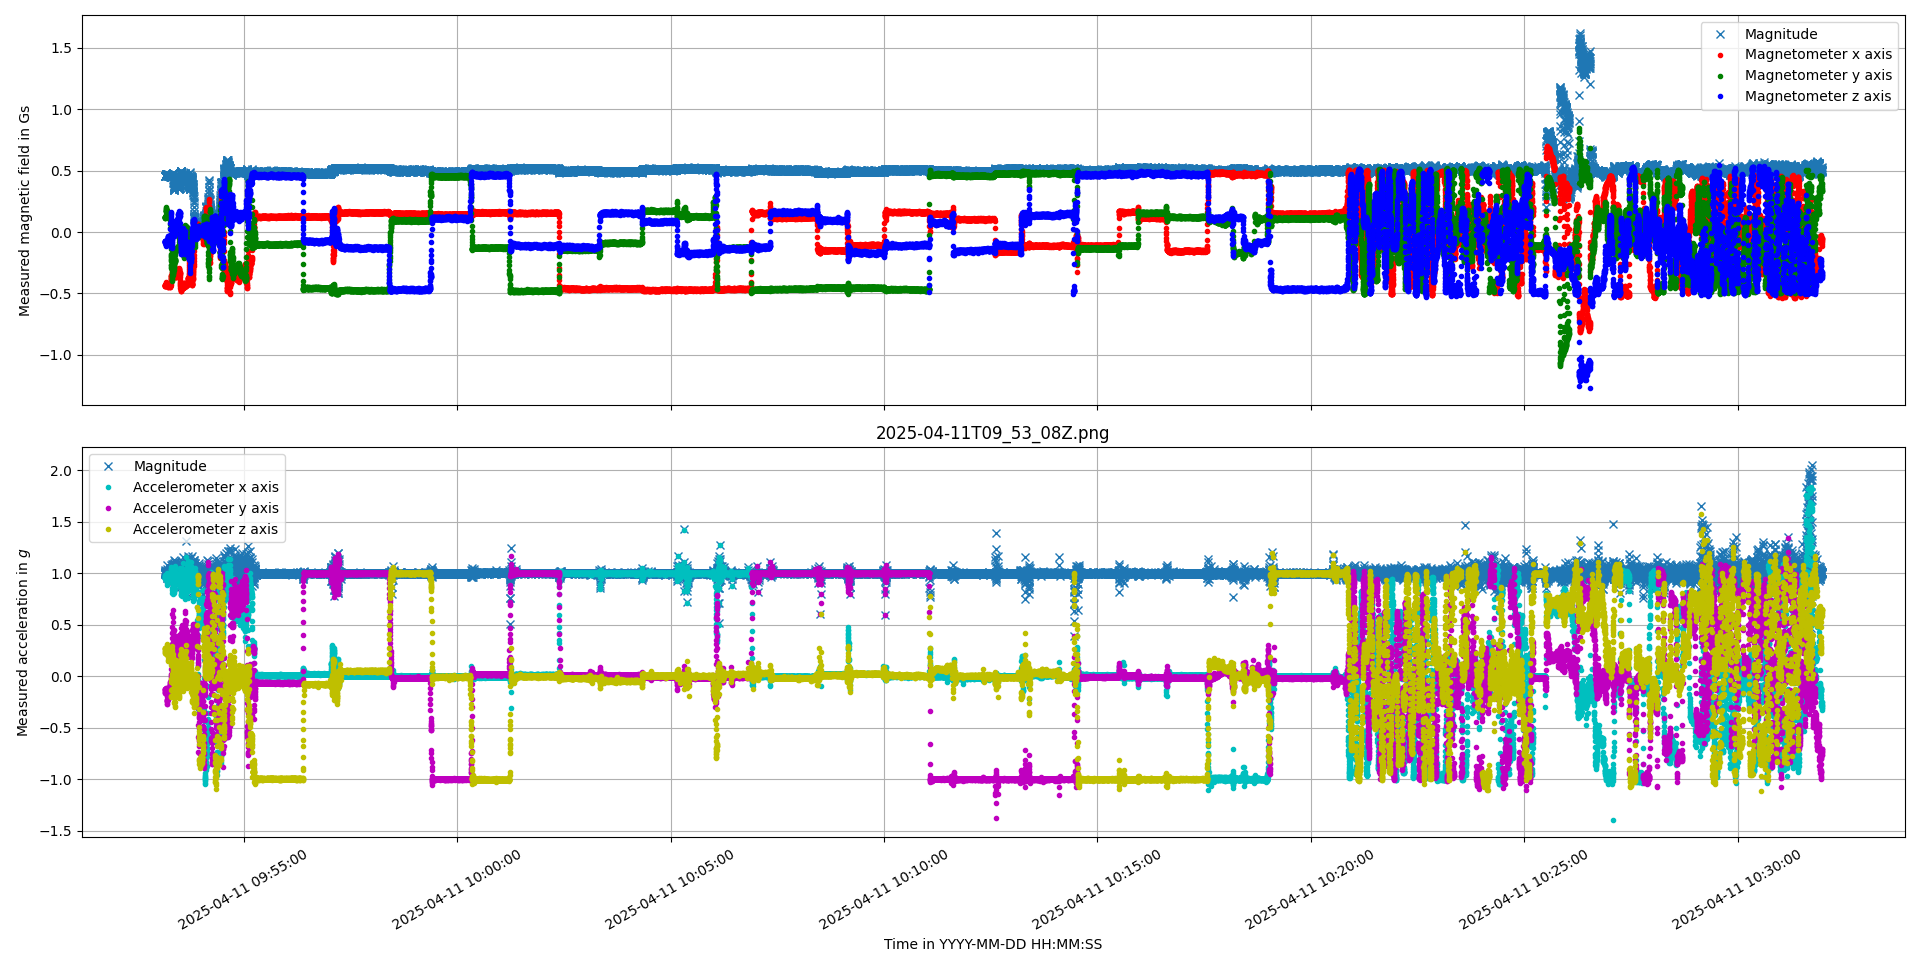
\includegraphics[width=\linewidth]{images/04_results/phaseii_calibrated_calibration11apr.png}
    \caption{Calibrated using coefficients from Phase II}
\end{figure}

\begin{figure}[H]
    \centering
    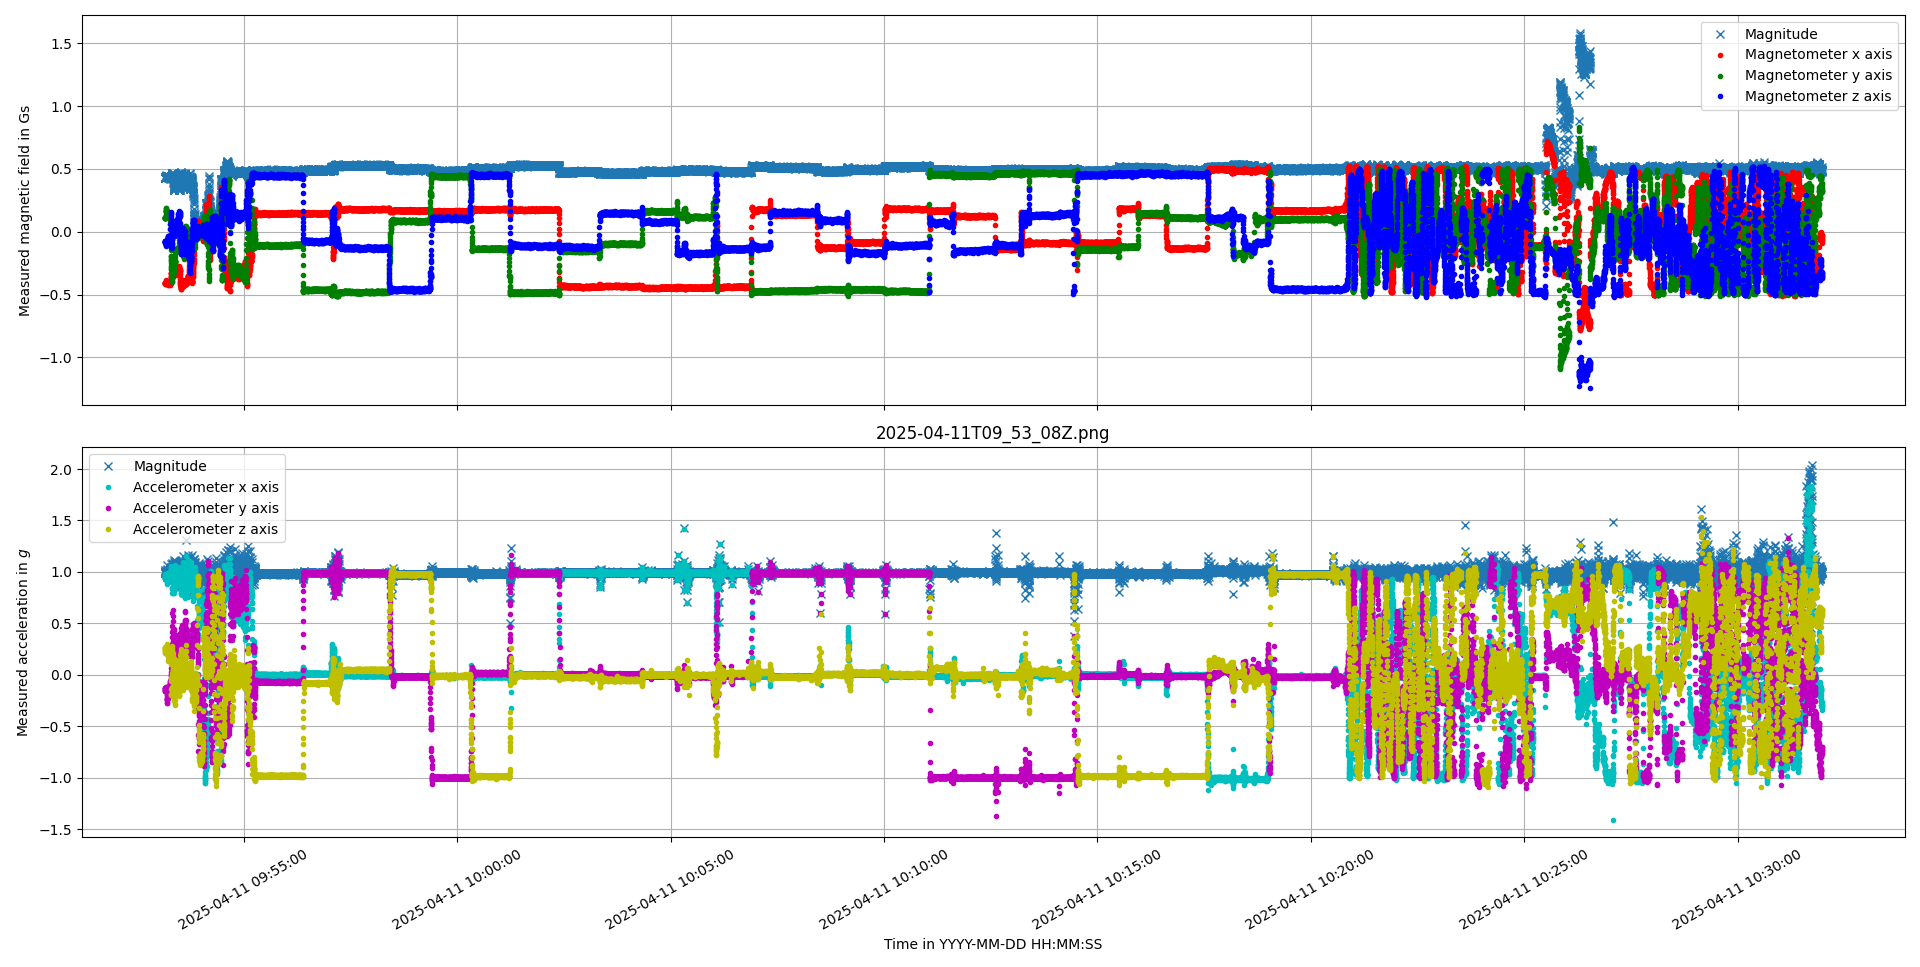
\includegraphics[width=\linewidth]{images/04_results/phaseiii_calibrated_calibration11apr.png}
    \caption{Calibrated using coefficients from Phase III}
\end{figure}

\begin{figure}[H]
    \centering
    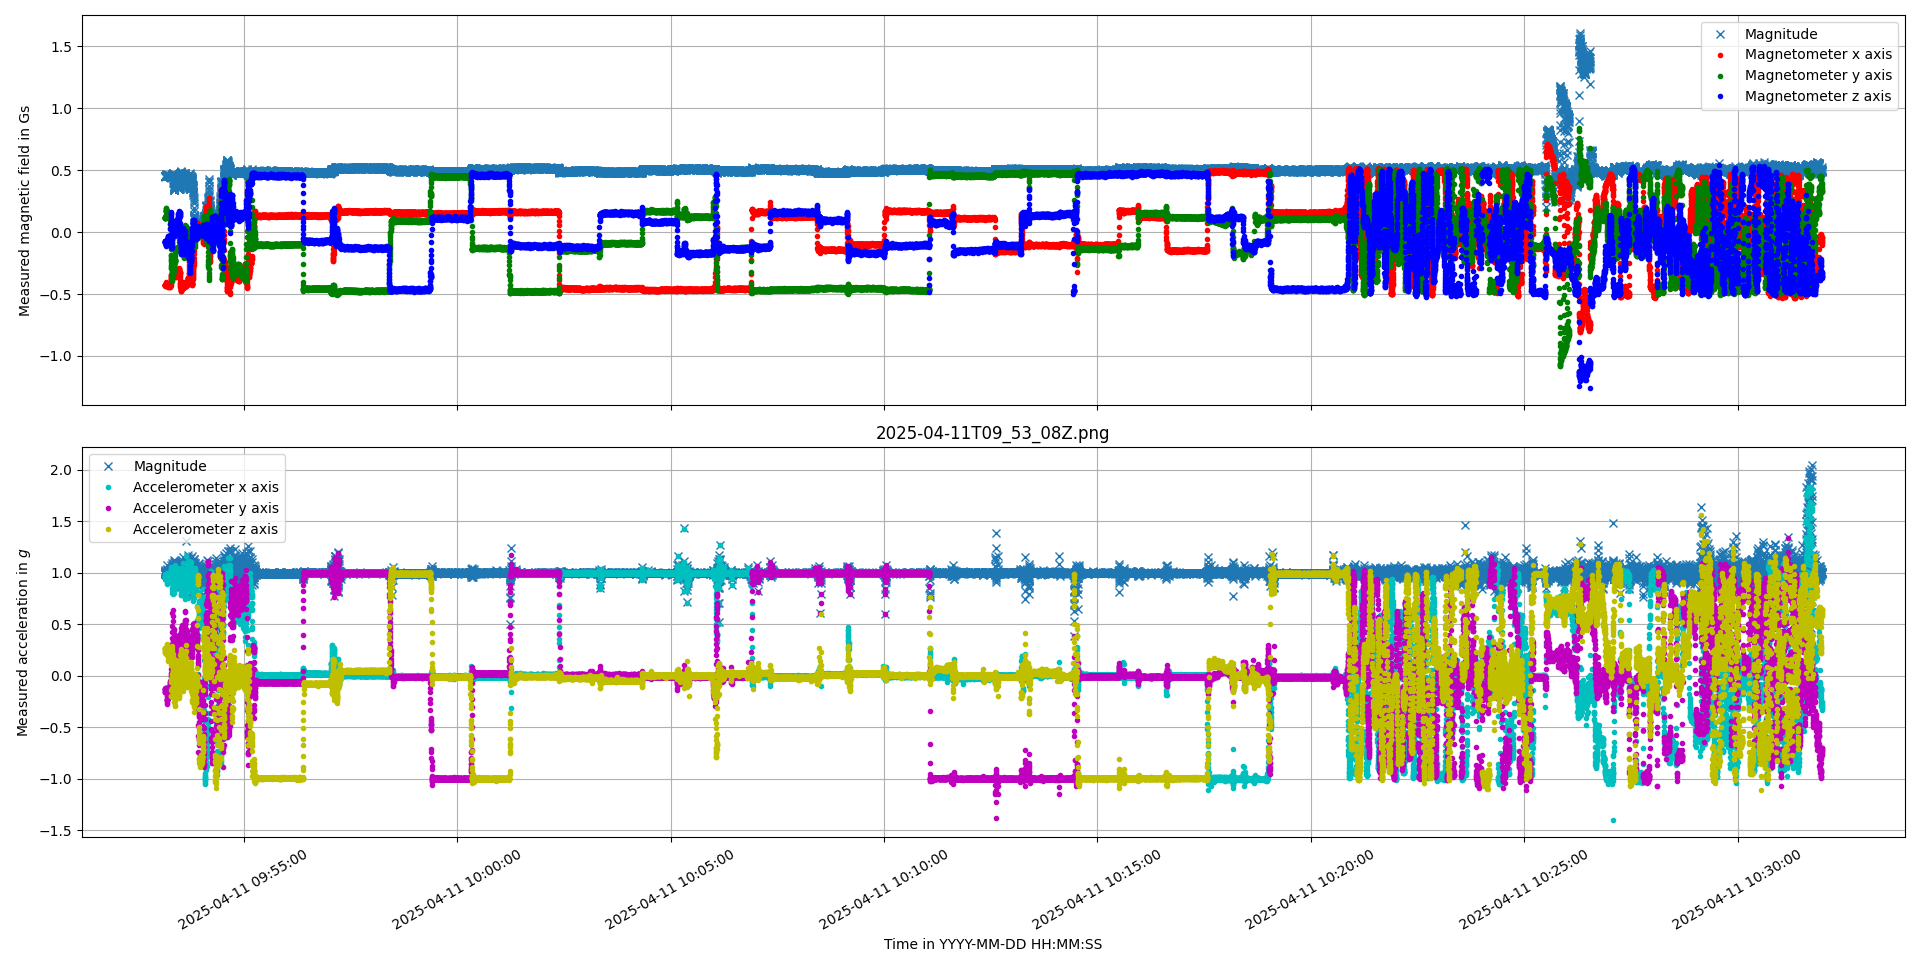
\includegraphics[width=\linewidth]{images/04_results/phaseii_and_iii_calibrated_calibration11apr.png}
    \caption{Calibrated using coefficients from Phases II and III}
\end{figure}


\chapter{Derivation of Coefficients \label{sec:app:deriv_of_coeff}}
The mathematical coefficients $a$, $b$, $c$, $x_0$, $y_0$ and~$z_0$ are to be related to the physical error matrices $C_{\mathrm{sf}}$, $C_\mathrm{zb}$, $C_\mathrm{si}$ and~$\delta\vec{B}$.

The mathematical equation is :
\begin{equation}
    \begin{pmatrix}B_{x,\ \mathrm{meas}} \\ B_{y,\ \mathrm{meas}}\\ B_{z,\ \mathrm{meas}} \end{pmatrix} = \begin{pmatrix} \frac{1}{\sqrt{a^B}} & 0 & 0 \\
                                                0 & \frac{1}{\sqrt{b^B}} & 0 \\
                                                0 & 0 & \frac{1}{\sqrt{c^B}}
                                                \end{pmatrix}\cdot\begin{pmatrix}
                                                    B_x \\ B_y \\ B_z
                                                \end{pmatrix}+\begin{pmatrix}
                                                    x_0^B \\ y_0^B \\ z_0^B
                                                \end{pmatrix}
\end{equation}

The Physical relation between measured and real field is:
\begin{equation}
    \begin{pmatrix}
    B_{x,\ \mathrm{meas}} \\
    B_{y,\ \mathrm{meas}} \\
    B_{z,\ \mathrm{meas}}
    \end{pmatrix}
    =
    \begin{pmatrix}
        c^\mathrm{sf}_z \\
        c^\mathrm{sf}_y \\
        c^\mathrm{sf}_z
    \end{pmatrix}
    \cdot
    \begin{pmatrix}
        c^\mathrm{si}_{11} & c^\mathrm{si}_{12} & c^\mathrm{si}_{13} \\
        c^\mathrm{si}_{21} & c^\mathrm{si}_{22} & c^\mathrm{si}_{23} \\
        c^\mathrm{si}_{31} & c^\mathrm{si}_{32} & c^\mathrm{si}_{33} 
    \end{pmatrix}
    \cdot \left\{
    \begin{pmatrix}
    B_x \\ B_y \\ B_z
    \end{pmatrix}
    +\begin{pmatrix}
     \delta B_x \\
     \delta B_y \\
     \delta B_z   
    \end{pmatrix} 
    \right\}
    +\begin{pmatrix}
        c^{\mathrm{zb}}_{11} & c^{\mathrm{zb}}_{12} & c^{\mathrm{zb}}_{13} \\
        c^{\mathrm{zb}}_{21} & c^{\mathrm{zb}}_{22} & c^{\mathrm{zb}}_{23} \\
        c^{\mathrm{zb}}_{31} & c^{\mathrm{zb}}_{32} & c^{\mathrm{zb}}_{33}
    \end{pmatrix}
\end{equation}

Now we simply compare the coefficients:
\begin{align}
    \begin{pmatrix}
    \frac{1}{\sqrt{a^B}} & 0 & 0 \\
    0 & \frac{1}{\sqrt{b^B}} & 0 \\
    0 & 0 & \frac{1}{\sqrt{c^B}}
    \end{pmatrix}
    =
    \begin{pmatrix}
        c^\mathrm{sf}_z \\
        c^\mathrm{sf}_y \\
        c^\mathrm{sf}_z
    \end{pmatrix}
    \cdot
    \begin{pmatrix}
        c^\mathrm{si}_{11} & c^\mathrm{si}_{12} & c^\mathrm{si}_{13} \\
        c^\mathrm{si}_{21} & c^\mathrm{si}_{22} & c^\mathrm{si}_{23} \\
        c^\mathrm{si}_{31} & c^\mathrm{si}_{32} & c^\mathrm{si}_{33} 
    \end{pmatrix}
\end{align}